\chapter{General Probability Spaces}

We will describe non-uniform distributions and the summation rules.

We will describe countable probability spaces, summable series, and
density distributions; all will be introduced through the idiom of the
rotating wheel that stops at a uniformly distributed angle.

\section{Distributions over the natural numbers}
%Akshay: I'm not sure what it means to work in the rotating wheel here, since random variables and their expectations (i.e. bets) haven't yet been considered, I believe.

Let's consider distributions over the positive integers $\mathbb{Z}^+ = \{1, 2, 3, \dots\}$. 
By now, we know that any valid probability distribution must have the total probability over all outcomes equal $1$. 
For a random variable $X$ over $\mathbb{Z}^+$, this means that
$$ \sum_{i=1}^\infty \pr(X = i) = 1 $$

Notice that the series is infinite, but it evaluates to a finite value. 
This can happen if the sum is a geometric series. 
If $\pr(X = i) = \frac{1}{2^i} $, for example, then $ \sum_{i=1}^\infty \pr(X = i) = \sum_{i=1}^\infty \frac{1}{2^i} = 1 $. 

However, other series have this property as well. 
One that will be useful to us is the series
$$ \sum_{i=1}^\infty \frac{1}{i^2} = \frac{\pi^2}{6} $$
%(Determining the value of this series was a famous mathematical problem for decades, called the Basel problem.)
Therefore, the distribution $\pr(X = i) = \frac{6}{\pi^2 i^2}$ is valid, because $ \frac{6}{\pi^2} \sum_{i=1}^\infty \frac{1}{i^2} = 1 $.

Of course, infinite series can evaluate to infinity as well. 
A well-known example we will use is the \emph{harmonic series}
$$ \sum_{i=1}^\infty \frac{1}{i} $$




\section{Tossing a biased coin}
\label{sec:BaisedCoin}

Suppose that instead of a fair coin, you have a coin whose probability of coming up heads is $p \in [0,1]$. The sample space for a single coin toss is $\Omega_o = \{H,T\}$ and the probabilities of the possible outcomes are
$$ \pr(H) = p, \ \ \pr(T) = 1-p.$$

If you toss this coin $n$ times (sample space $\Omega = \{H,T\}^n$), what is the chance of getting exactly $k$ heads? Well, pick any sequence $\omega \in \Omega$ with $k$ heads. The probability of getting precisely the outcome $\omega$ is
$$ \pr(\omega) = p^k (1-p)^{n-k} .$$
Thus the probability of $k$ heads is
$$ \mbox{(number of sequences with $k$ heads)} \cdot p^k (1-p)^{n-k} 
\ \ = \ \ 
{n \choose k} p^k (1-p)^{n-k} .$$

Sometimes we encode heads and tails numerically:
$$ \mbox{heads} \rightarrow 1, \ \ \ \mbox{tails} \rightarrow 0 .$$

In this case, a single coin flip with bias $p$ has sample space $\{0,1\}$ and is called a Bernoulli($p$) distribution. Suppose $n$ such coins are flipped, and $X_i \in \{0,1\}$ is the outcome for the $i$th coin. Then the number of heads is simply 
$$ X = X_1 + X_2 + \cdots + X_n. $$
$X$ has sample space $\{0,1,\ldots,n\}$ and is said to have a Binomial($n,p$) distribution.


\section{Throw a dart at a dartboard} 

Suppose for convenience that your dartboard has radius 1, and is
centered at the origin. Its bullseye has radius 0.1. You throw a dart
at it, which lands at a random location (all positions on the board
are equally likely). What is the chance that it lands exactly at the
origin? What is the chance that it lands in the bullseye?

This differs from earlier examples in that the sample space is infinite and continuous. It is the set of all possible locations of the dart: any point in the circle. We can represent any such point by its $(x,y)$ coordinates: $\Omega = \{(x,y): x^2 + y^2 \leq 1\}$.

The chance of landing exactly at the origin is 0, since there are infinitely many places the dart could land. It makes more sense to talk about landing in {\it regions} $A \subset \Omega$ rather than specific points $\omega \in \Omega$. In general
$$ \pr(A) = \frac{\mbox{area of $A$}}{\mbox{area of $\Omega$}} $$
and therefore $\pr(\mbox{bullseye}) = (0.1)^2 = 0.01$.

\section{Cumulative Distribution Functions}

Our discussion so far focused on finite event spaces or event spaces
that correspond to the integers $0,1,2,\ldots$ (so-called countable
infinite sets). How do we define distributions over the real numbers?
That is an {\em uncountably} infinite set.\footnote{A set $A$ is
  uncountable if there is no one-to-one mapping from $A$ to the
  positive integers $1,2,3,4,...$. In other words, a set is
  uncountable if you cannot create a list which includes all of the
  elements in the set.}

When defining a distribution over the real it is not enough to assign
probabilities to individual points on the real line. Consider the {\em
  uniform distribution on the line segment $[0,1]$}, by which
we mean the set $\{x | 0 \leq x \leq 1\}$. We cannot assign each
point a probability larger than zero. because that would result in
$[0,1]$ an infinite probability. What we do instead is assign
probability to the line segment $0 \leq a < b \leq 1$ the probability
$b-a$. Thus for example $P([1/4,1/3])=1/3-1/4 = 1/12$.

More generally, we can define any distribution over the real line
using the {\em Cumulative Distribution Function}:
\[
\CDF(a) \doteq P(x \leq a)
\]

\begin{figure}[th]
\begin{center}
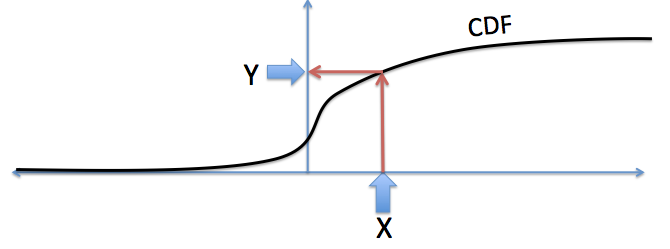
\includegraphics[width=5in]{figs/CDFmapping.png}
\end{center}
\caption{This figure depicts an example of mapping a random variable
  $X$ whose distribution is defined by a CDF (thick black curve) to
  another random variable $Y$, whose distribution is uniform in the
  interval $[0,1]$. The mapping uses the CDF as a function so that
  $Y=\CDF(X)$. \label{fig:CDFmap}}
\end{figure}

\begin{figure}[h]
\begin{center}
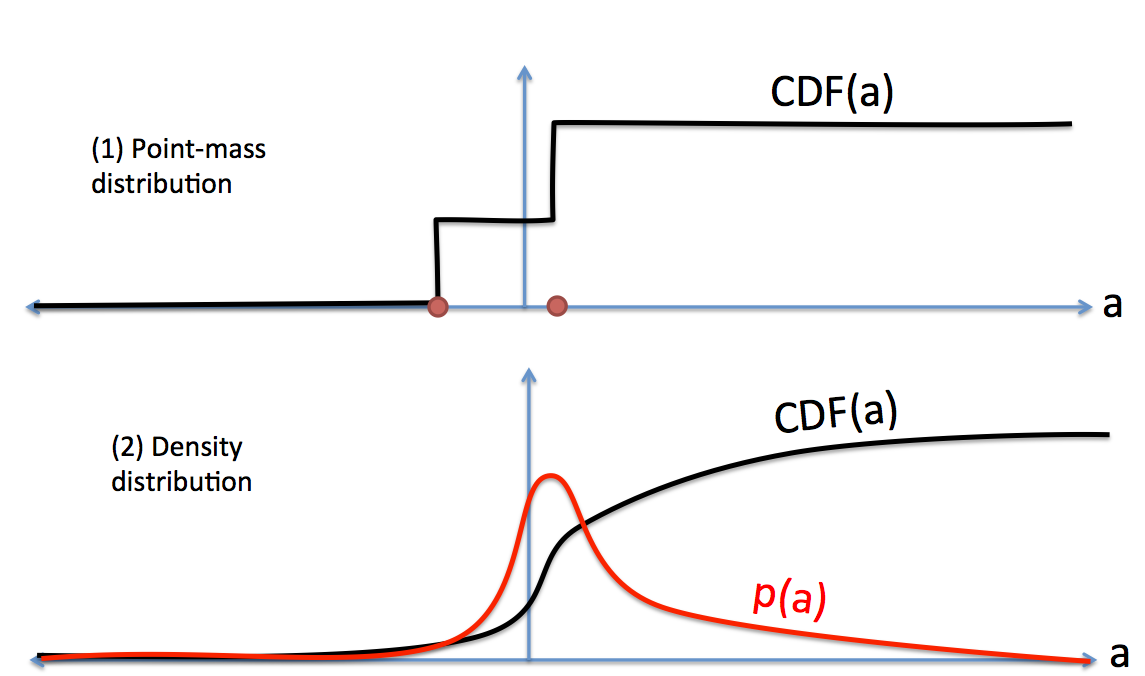
\includegraphics[width=5in]{figs/CDFs.png}
\end{center}
\caption{The CDFs for two distributions: (1) A point-mass distribution
  is a distribution that assignes non zero probabilities to two real
  values (marked by red circles) all sets that do not include at least
  one of these points have probability zero. The CDF of a point mass
  distribution is constant every where but at the point masses where
  it is discontinuous, the size of the discontinuity is the
  probability of the corresponding point. (2) A density distribution
  assigns probability zero to any single point. The CDF for such a
  distribution is a continuous increasing function that has a
  derivative. This derivative, $p(a)$ is called the {\em density function} of
  the distribution. For density distributions the CDF and the density
  function contain the same information.\label{fig:CDF}}
\end{figure}

As we see in Figure~\ref{fig:CDF} the CDF is an increasing function that
increases from zero at $-\infty$ to one at $+\infty$.

It is easy to see that $P(a<x\leq b)=\CDF(b)-\CDF(a)$.


\section{Examples of distributions on the real line}
If the distribution assigns a non-zero probability to some $x=a$ we
say that the distribution has a {\em point mass} at $a$. In that case
the $\CDF$ has a jump at $a$. We denote a point mass distribution
concentrated at the point $a$ by $PM(a)$. The distribution $PM(a)$
corresponds to a random variable such that $P(X=a)=1$.

\begin{figure}[t]
\begin{center}
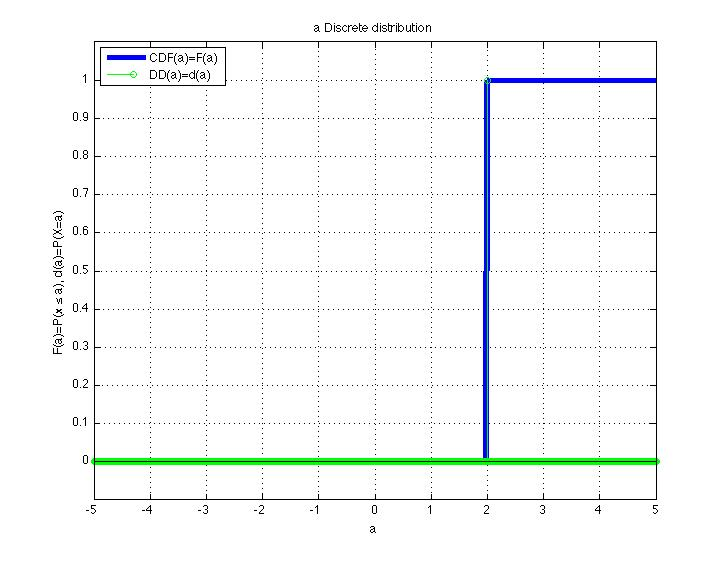
\includegraphics[width=3in]{figs/Discrete1.jpg}
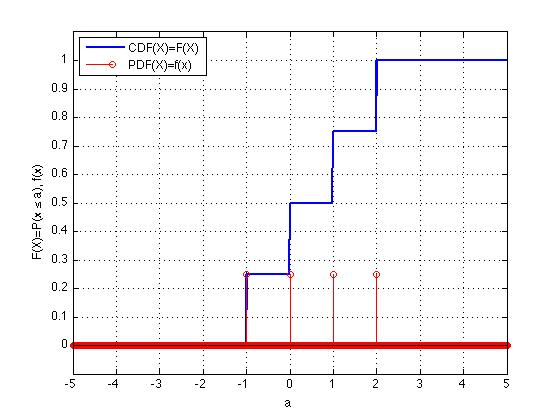
\includegraphics[width=3in]{figs/4PointMass.jpg}
\end{center}
\caption{{\bf Left:} A discrete distribution concentrated on a single
  point $P(X=2)=1$. We denote this distribution by $PM(2)$.  {\bf
    Right:} A discrete distribution distributed evenly over the four
  points $-1,0,1,2$. This distribution can be expressed as $(PM(-1)+PM(0)+PM(1)+PM(2))/4$.}
\end{figure}

\begin{figure}[b]
\begin{center}
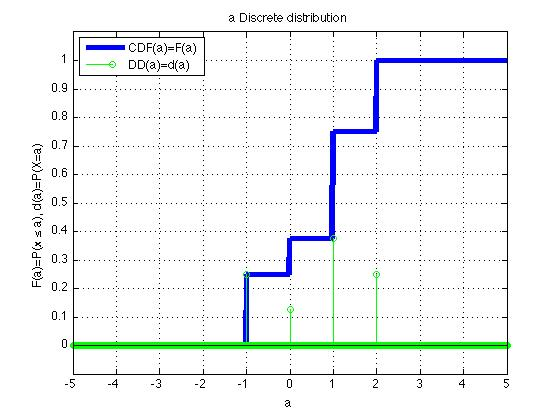
\includegraphics[width=3in]{figs/Discrete2.jpg}
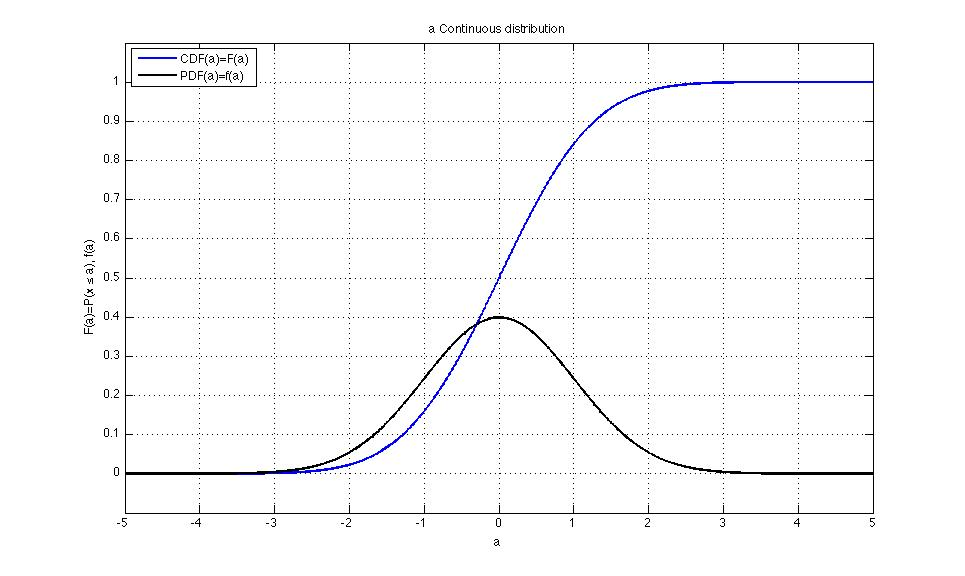
\includegraphics[width=3in]{figs/Normal.jpg}
\end{center}
\caption{{\bf Left:} A non-uniform discrete distribution. This
  distribution can be expressed as
  $(1/4)PM(-1)+(1/8)PM(0)+(5/8)PM(1)+(1/4)PM(2)$. {\bf Right:} The
  normal distribution with mean $0$ and varriance 1, denoted ${\cal
  N}(0,1)$. This is a density distribution and it's density function
is $f(x) = \frac{1}{\sqrt{2\pi}} \exp(-x^2/2)$.}
\end{figure}

\begin{figure}[t]
\begin{center}
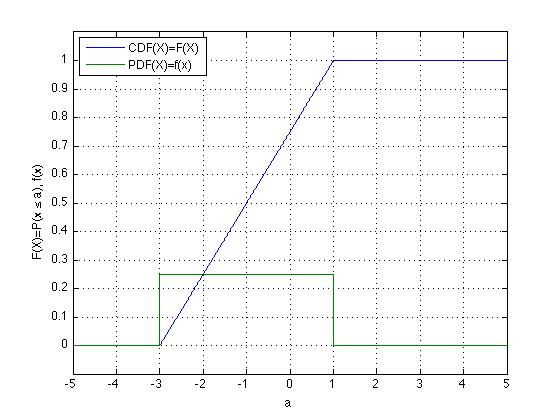
\includegraphics[width=3in]{figs/Uniform.jpg}
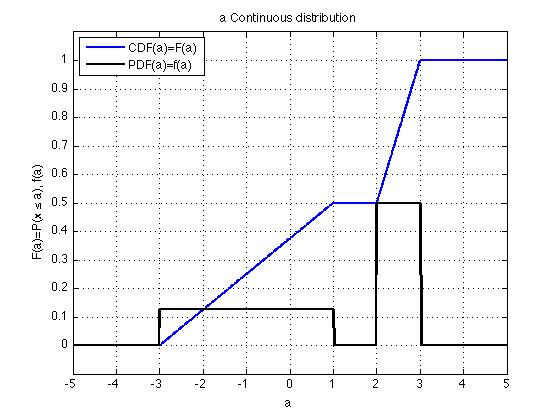
\includegraphics[width=3in]{figs/unifMixture2CDF.jpg}
\end{center}
\caption{{\bf Left:} A uniform distribution between $-3$ and $1$. We
  denote this distribution by $U(-3,1)$. {\bf Right:} A mixture of two
  uniform distributions: $(U(-3,1)+U(2,3))/2$.}
\end{figure}

\[
f(x) = \begin{cases}
0.25 & \mbox{if $ -3 \leq x \leq 1$} \\
0 & \mbox{otherwise}
\end{cases}
\]

Another important case is when the deriveative of the CDF is deifined
$p(a) = \frac{d}{dx}\left|_{x=a} \CDF(x)\right.$. The function $p(a)$
is called the {\em probability density}. Note that if $p(a)$ is
defined then, regarless of how large $p(a)$ is, $P(x=a)=0$.

When a distribution over the reals is a density distribution we can
calculate the probability of the segment $[a,b]$ using the integral:
\[
P(a < x \leq b)=\CDF(b)-\CDF(a)=\int_a^b p(x) dx
\]

